\section{Results}
\label{sec:results}

All data in this section are produced by the experiment runner
\texttt{sph\_experiments} and plotted by the script
\texttt{plots/make\_plots.py}; rerunning both regenerates every figure.

\subsection{Correctness Tests}

The repository includes CTest unit tests for the neighbour search, for the
density summation (an isolated particle carries $m\,W(0,h)$; a particle inside a
regular lattice recovers $\rho_0$ to within $0.01\,\%$), for the slope of the
equation of state ($\partial p/\partial\rho = c^2$ at $\rho_0$), and a short
hydrostatic-column regression test that checks the CFL limit, containment, the
density error and the hydrostatic pressure profile.

\subsection{Hydrostatic Column}

Figure~\ref{fig:hydro-pressure} compares the particle pressures of the settled
column with the hydrostatic solution $p = \rho_0 g d$. Instantaneous pressures
scatter around the solution with a mean deviation of about $10\,\%$ of
$\rho_0 g H$. Averaged over $2\,\mathrm{s}$, the scatter shrinks to $2.4\,\%$
and the mean pressure below the surface layer matches the hydrostatic value to
within $0.3\,\%$. The instantaneous scatter is therefore not a bias but acoustic
noise: pressure waves travel through the column much faster than the frame
rate.

\begin{figure}[ht]
    \centering
    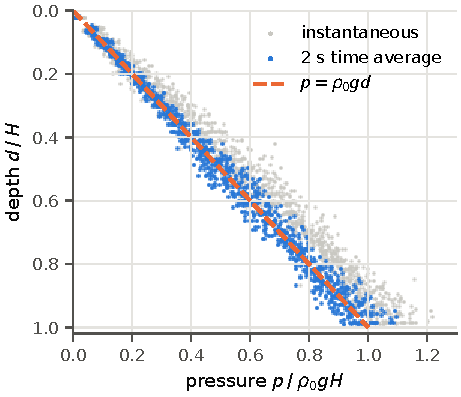
\includegraphics{figures/hydro_pressure.pdf}
    \caption{Pressure against depth in the settled hydrostatic column
    ($t = 8$--$10\,\mathrm{s}$). Grey: instantaneous particle pressures; blue:
    pressures averaged over $2\,\mathrm{s}$; dashed: hydrostatic solution.}
    \label{fig:hydro-pressure}
\end{figure}

Figure~\ref{fig:hydro-settling} shows how the column settles. The particles
start on a lattice at exactly $\rho_0$ and therefore without pressure, so the
column first falls slightly and then oscillates acoustically. Viscosity damps
the mean kinetic energy by more than an order of magnitude within
$10\,\mathrm{s}$. The maximum density error settles at $0.56\,\%$ (mean
$0.25\,\%$), close to the estimate $\Delta\rho/\rho_0 \approx gH/c^2 = 0.5\,\%$
for the compression at the bottom of the column. The adaptive time step settles
at $\Delta t \approx 1.2\times10^{-3}\,\mathrm{s}$, i.e.\ 13 substeps per frame.

\begin{figure}[ht]
    \centering
    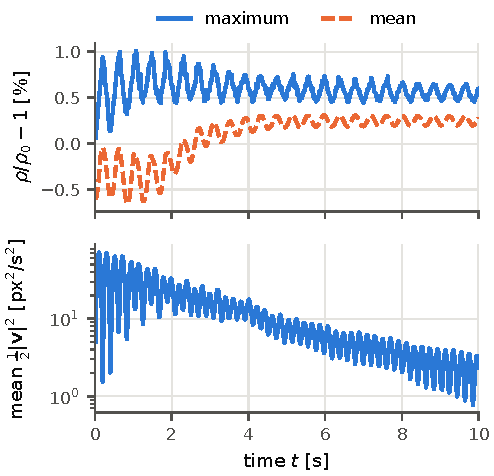
\includegraphics{figures/hydro_settling.pdf}
    \caption{Settling of the hydrostatic column: density error (top) and mean
    kinetic energy per unit mass (bottom, logarithmic).}
    \label{fig:hydro-settling}
\end{figure}

\subsection{Dam Break}

Figure~\ref{fig:dam-snapshots} shows the collapse of the water column, coloured
by pressure. The front position $Z$ along the floor is shown in
Fig.~\ref{fig:dam-front} in the dimensionless form of Martin and
Moyce~\cite{martin1952}. The front reaches $Z/a = 1.87$ at $T = 1$ and
$3.62$ at $T = 2$, and hits the opposite wall ($Z/a = 4$) at $T = 2.18$. After
an initial acceleration phase the front moves at a nearly constant speed. The
shallow-water solution of Ritter~\cite{ritter1892}, $Z/a = 1 + 2nT$, assumes
that the front starts at full speed and bounds the motion from above.
% TODO: add the Martin & Moyce comparison once Latex/data/martin_moyce_n2.csv is
% filled in; SPH fronts are commonly reported to run ahead of the experiment.

\begin{figure}[ht]
    \centering
    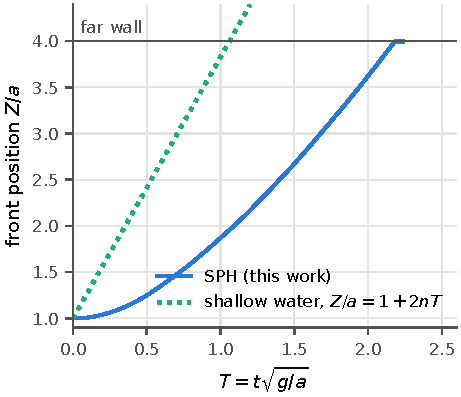
\includegraphics{figures/dam_front.pdf}
    \caption{Front position of the dam break in dimensionless form
    ($a$: initial column width, $n^2 = H/a = 2$).}
    \label{fig:dam-front}
\end{figure}

\begin{figure}[ht]
    \centering
    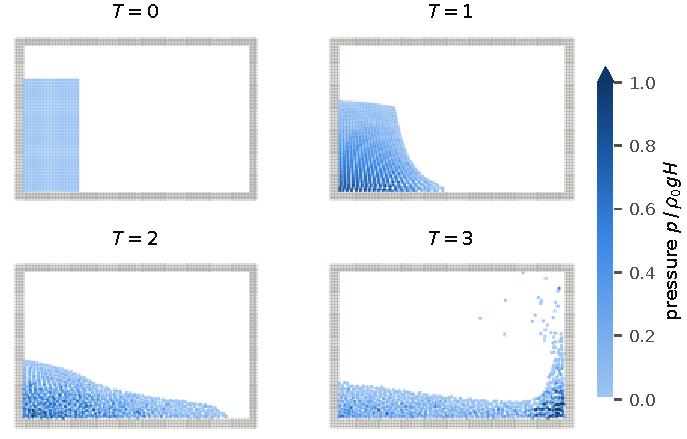
\includegraphics{figures/dam_snapshots.pdf}
    \caption{Dam break at $T = t\sqrt{g/a} = 0, 1, 2, 3$. Fluid particles are
    coloured by pressure, smoothed over $0.05\,\mathrm{s}$ per particle to
    suppress acoustic noise; wall particles are grey.}
    \label{fig:dam-snapshots}
\end{figure}

Until the impact on the right wall the maximum density error stays below
$1.5\,\%$ and the Mach number below $0.11$, as intended by the choice of $c$. At
the impact the flow is deflected upwards and the splash reaches
$\mathrm{Ma} = 0.23$, more than twice the free-fall estimate; the density error
peaks at $8.9\,\%$ for a few frames. The speed of sound chosen from a free-fall
estimate is therefore adequate for the collapse itself but marginal for the
impact.

\subsection{Speed of Sound}

The speed of sound trades compressibility against cost
(Fig.~\ref{fig:sweep-c}). Doubling $c$ reduces the density error of the
hydrostatic column roughly fourfold ($10.2\,\%$, $3.0\,\%$, $0.75\,\%$ and
$0.35\,\%$ for $c/\sqrt{2gH} = 2.5, 5, 10, 20$), following the $gH/c^2$ estimate
until noise dominates at the stiffest setting. In the dam break, the time-averaged peak density error
decreases only proportionally to $1/c$ ($8.1\,\%$ to $0.8\,\%$), because it is
set by local dynamic compression rather than by the hydrostatic load. The
number of substeps grows almost in proportion to $c$ (from 5 to 28 per frame
for an eightfold increase) since the acoustic CFL condition dominates. A stiffer fluid is also noisier: the
frame-to-frame pressure change grows from $2.3\,\%$ to $40\,\%$ of $\rho_0 g H$,
because the same small density fluctuation is multiplied by $B \propto c^2$.
The front position is insensitive to $c$ ($Z/a$ at $T = 1.5$ varies by less than
$1\,\%$).

\begin{figure}[ht]
    \centering
    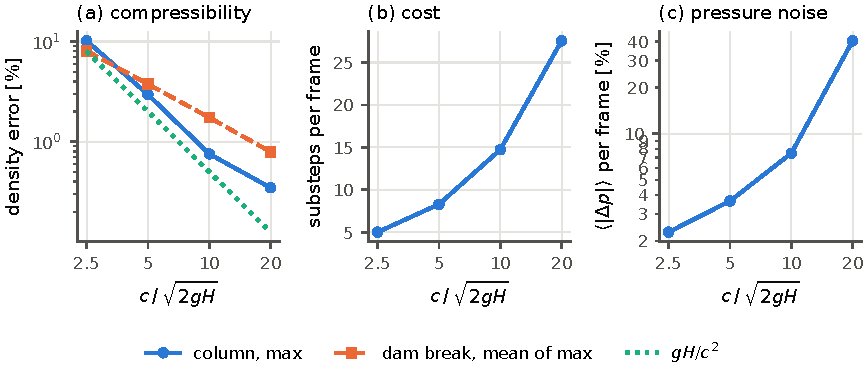
\includegraphics{figures/sweep_speed_of_sound.pdf}
    \caption{Influence of the speed of sound: (a) density error with the
    hydrostatic estimate $gH/c^2$, (b) substeps per $1/60\,\mathrm{s}$ frame
    in the dam break, (c) mean frame-to-frame pressure change in the settled
    column.}
    \label{fig:sweep-c}
\end{figure}

\subsection{Viscosity}

Viscosity mainly controls the acoustic noise (Fig.~\ref{fig:sweep-visc}). With
$\nu = 50$ the instantaneous pressure of the settled column deviates by $51\,\%$
from the hydrostatic value on average; $\nu = 150$ reduces this to $10\,\%$.
Larger viscosities do not reduce the instantaneous error further ($15$--$17\,\%$),
while the time-averaged error stays between $1.5$ and $3.2\,\%$ for all values.
The flow itself becomes slower with increasing viscosity: at $T = 1.5$ the front
has reached $Z/a = 2.74$ for $\nu = 50$ and $2.53$ for $\nu = 1000$. The default
$\nu = 150$ is a compromise between noise and numerical dissipation.

\begin{figure}[ht]
    \centering
    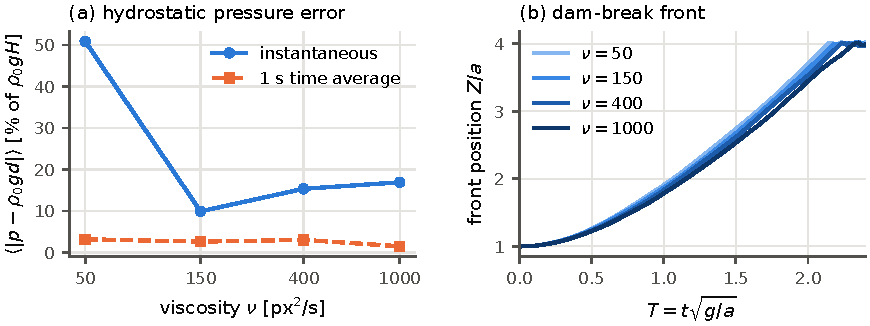
\includegraphics{figures/sweep_viscosity.pdf}
    \caption{Influence of the viscosity $\nu$: (a) mean pressure error of the
    settled column, instantaneous and averaged over $1\,\mathrm{s}$; (b) front
    position of the dam break.}
    \label{fig:sweep-visc}
\end{figure}

\subsection{Kernel Support and Pairing Instability}
\label{sec:pairing}

Figure~\ref{fig:pairing} shows how the ratio $h/\Delta x$ changes the particle
arrangement in the settled column. At $h/\Delta x = 1.2$ the particles remain
on the initial lattice, visible as sharp peaks every $10\,\mathrm{px}$; the
fluid behaves like a crystal. At $1.3$ the particles rearrange into a
disordered, liquid-like state. At $1.6$ and $2.0$ (33 and 50 neighbours instead of
about 20) the particles collapse into horizontal rows $18$--$20\,\mathrm{px}$
apart, roughly twice the initial spacing, while the spacing within a row shrinks:
the pairing instability of the cubic spline \cite{dehnen2012}. The rows also
make the pressure noisier: at $h/\Delta x = 2.0$ the frame-to-frame pressure
change is four times larger than at $1.3$. The front position of the dam break
is not affected by the ratio.

\begin{figure}[ht]
    \centering
    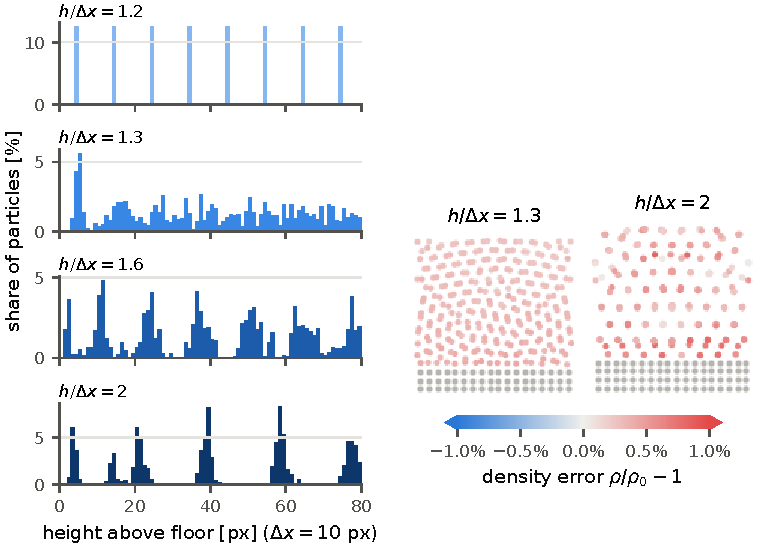
\includegraphics{figures/pairing.pdf}
    \caption{Particle arrangement in the settled hydrostatic column for
    different $h/\Delta x$. Left: distribution of particle heights above the
    floor (1\,px bins, central region). Right: the bottom of the column for
    $h/\Delta x = 1.3$ and $2.0$, coloured by density error.}
    \label{fig:pairing}
\end{figure}

\subsection{Density Fields}

Figure~\ref{fig:density-grid} compares the density error of the dam break at
$T = 2$ for all parameter variations. With $c = 2.5\sqrt{2gH}$ the lower part of
the fluid is compressed by several percent; from $c = 10\sqrt{2gH}$ on, the bulk
is within about $\pm1\,\%$ of $\rho_0$. In all runs the free surface shows a
density deficit, because the kernel support of surface particles is only
partially filled. Viscosity and $h/\Delta x$ hardly change the density field
at this resolution.

\begin{figure}[ht]
    \centering
    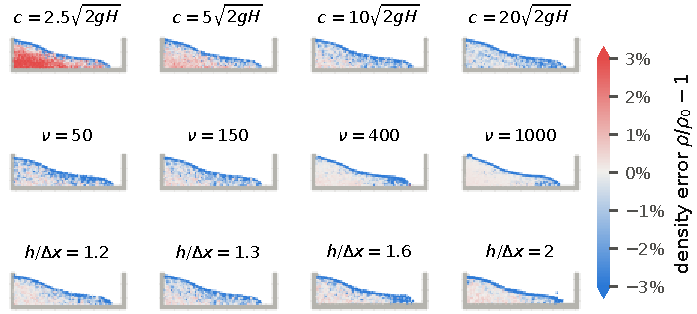
\includegraphics{figures/density_grid.pdf}
    \caption{Density error $\rho/\rho_0 - 1$ in the dam break at $T = 2$ (lower
    part of the tank). Rows vary the speed of sound, the viscosity, and the
    ratio $h/\Delta x$; the default setup is $c = 10\sqrt{2gH}$, $\nu = 150$,
    $h/\Delta x = 1.3$.}
    \label{fig:density-grid}
\end{figure}

\subsection{Discussion}

The weakly compressible model reproduces the hydrostatic pressure with a
time-averaged accuracy of a few percent and keeps density errors at about one
percent for the chosen speed of sound. Its main weakness is acoustic pressure
noise: instantaneous particle pressures scatter by about $10\,\%$ of the
hydrostatic pressure even in a fluid at rest. The interactive renderer
therefore colours particles by a per-particle moving average of the pressure.
Methods that diffuse density perturbations ($\delta$-SPH) or solve for pressure
implicitly (IISPH, DFSPH) would remove this noise at the source.

Further limitations are the $\mathcal{O}(N^2)$ neighbour search, which limits
the resolution to about $10^3$ fluid particles at interactive rates; the
projection safety net at the walls, which is not part of the SPH formulation;
and the free-fall estimate of the flow speed used to choose $c$, which
underestimates the speeds reached at the wall impact.
